\documentclass[a4paper,12pt]{article}
\usepackage[a4paper, margin=2.4cm]{geometry}
\usepackage[utf8]{inputenc}
\usepackage{amsmath, amssymb} % Packages pour les maths
\usepackage[T1]{fontenc}
\usepackage{graphicx} 
\usepackage{caption}
\usepackage{setspace} % Espacement des lignes
\usepackage{tikz}
\usepackage{soul}
\usepackage{titlesec}
\titleformat*{\section}{\LARGE\bfseries}
\titleformat*{\subsection}{\Large\bfseries}
\titleformat*{\subsubsection}{\normalsize\bfseries}
\begin{document}
\section*{Modèle 2: Avec atmosphère}
\subsection*{1. Boule d'eau avec atmosphère }
\subsubsection*{Hypothèses}:
\begin{itemize}
    \item Terre assimilé à boule d'eau, de température \(T_{\text{Terre}}\) 
    \item  Atmosphère avec une température uniforme T 
    \item  Sans puissance solaire reçue  
    \item  Ignorance de la convection  
    \item \(c_m=c_{\text{m,Terre}}\sim c_{\text{m,eau}}\) 
    \item $T(t=0) = T_i$ \ \ \
$T(t \to +\infty) = T_0$
    \item La Terre ne rayonne pas
   
\end{itemize}

\subsubsection*{Schéma:} 
\noindent\textcolor{gray}{\rule{\linewidth}{0.4pt}}

    
\begin{center}
  \input{modele2/figures/Schéma mathcha modèle 2.1.txt}
\end{center}
\noindent\textcolor{gray}{\rule{\linewidth}{0.4pt}}

\subsubsection*{Équations de transfert thermique}

On applique le premier principe appliqué au système \{ boule d'eau  \}

\begin{align*}
\delta Q &= C\, dT = -P_{\text{th,cond}} \cdot dt \\
\Rightarrow -\int \int \vec{j_{\text{th,cond}}}\, \vec{dS}\,dt = C\, dT \\
\Rightarrow -\int_{\theta=0}^\pi \int_{\phi=0}^{2\pi} h(T - T_0) \vec{e_{\text{r}}}\cdot r^2 \sin\theta\, d\theta\, d\varphi \vec{e_{\text{r}}}\, dt &=  C\, dT  \\
\Rightarrow -h(T - T_0) \cdot 4\pi\, dt &= C\, dT \\
\Rightarrow -T + T_0 = \frac{C}{h 4\pi} \frac{dT}{dt} \Rightarrow \frac{dT}{dt} &= -\frac{4\pi h}{C}(T - T_0)
\end{align*}

\vspace{0.5cm}

\subsubsection*{Solution:} 
$T(t) = T_0 + (T_i - T_0)e^{-kt}$ \quad avec $k = \frac{4\pi h}{C}$
\\
\bigskip
\subsubsection*{Modélisation graphique :} 
\begin{center}
  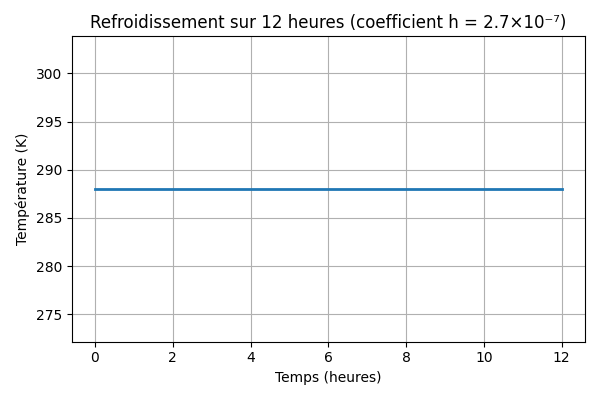
\includegraphics[width=0.8\linewidth]{../modele2/figures/modele2.png}
\end{center}
    

\subsection*{2. Coquille assimilée à de l'eau avec atmosphère }
\subsubsection*{Hypothèses}:
\begin{itemize}
    \item On garde les hypothèses précédente excepté le système: la Terre est assimilée à une coquille d'eau, d'épaisseur dr, avec du vide à l'intérieur de la coquille \end{itemize}

\subsubsection*{Schéma:} 
\noindent\textcolor{gray}{\rule{\linewidth}{0.4pt}}

    
\begin{center}
  \input{modele2/figures/Schéma modèle 2.2 coquille.txt}
\end{center}
\noindent\textcolor{gray}{\rule{\linewidth}{0.4pt}}
\subsubsection*{Modélisation graphique :} 
\begin{center}
  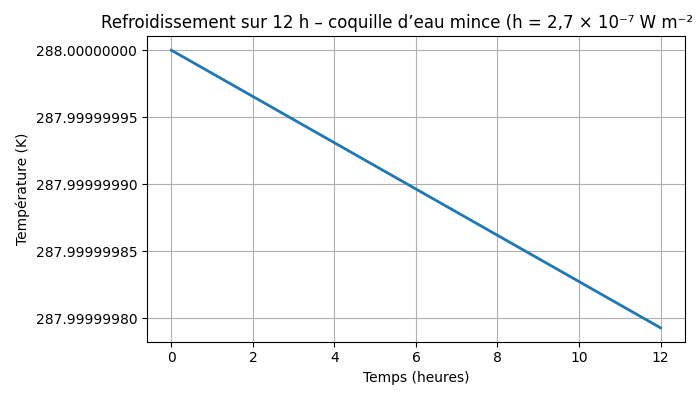
\includegraphics[width=0.8\linewidth]{../modele2/figures/modele2_coquille.png}
\end{center}
        


\subsection*{Critique du modèle}

\begin{itemize}
    \item Température de la Terre subjective.
    \item Épaisseur de la coquille.
    \item Prise en compte de l’atmosphère donc utilisation de la loi de Newton :
    \begin{itemize}
        \item MAIS problème de définition de la couche limite puisqu’on ne souhaite pas prendre en compte la convection pour le moment.
    \end{itemize}
    \item Dans les codes \texttt{modele2\_coquille.py} et \texttt{modele2\_boule.py}, on a posé $h = \lambda_{\text{air}} / \delta$ avec $\lambda_{\text{air}} = 0{,}027 \, \mathrm{W/(K \cdot m)}$.
    \begin{itemize}
        \item On a pris $\delta = 100\, \mathrm{km}$ comme longueur de la couche limite pour ne pas se préoccuper de la convection avant la thermosphère (85 km – 600 km).
        \item Mais cette hypothèse ne semble pas pertinente, puisque la loi de Newton est adaptée à un modèle conducto-convectif.
        \item On peut donc prendre un $\delta$ plus raisonnable, de l’ordre de 50 cm.
    \end{itemize}
    \item Problème de définition de $T_0$ :
    \begin{itemize}
        \item Si on suit notre modèle, ce serait la température au-delà de la thermosphère.
        \item Or on a posé $T_0 = 273\, \mathrm{K}$ dans nos codes Python.
    \end{itemize}
\end{itemize}

\end{document}